Link cut tree é uma estrutura de dados que representa uma floresta de árvores enraizadas. Cada árvore na floresta é um caminho disjunto de vértices (caminho preferencial), onde cada caminho é representado por uma esturtura de dados auxiliar, no nosso caso usaremos a Splay tree.  

Os nós na estrutura de dados auxiliar são ordenados de acordo a sua profundidade na Link cut tree. Desta forma, em uma splay tree podemos verificar que um nó é mais profundo que seu pai se for filho direito, e será mais superficial se for filho esquerdo.~\cite{WikipediaLCT}  

Na imagem a seguir temos como a Link cut tree representa os caminhos disjuntos de vértices em uma floresta de árvores enraizadas.
\begin{figure}
    \centering
    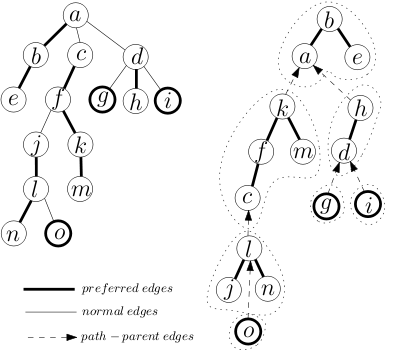
\includegraphics[width=7cm]{lct.png}
    \caption{Exemplo de Link cut tree. (Pega no wikipedia)}
\end{figure}

As rotinas usadas na implementação da Link cut tree foram:  
\begin{verbatim}
    Node maketree();
    void link(Node, Node);
    void cut(Node);
    void access(Node);
    Node findRoot(Node);
    void evert(Node);
\end{verbatim}

\begin{itemize}
    \item \texttt{maketree()}: retorna a raíz de uma link cut tree com apenas um nó, tendo complexidade de $O(1)$ em tempo.  
    \item \texttt{link(v, w)}: assumimos que \texttt{v} e \texttt{w} estão em árvores distintas. Nesta rotina acrescentaremos a aresta \texttt{vw} \textcolor{red}{(ou \texttt{wv}??)}, fazendo com que \texttt{v} seja pai de \texttt{w}. Esta rotina tem complexidade O(access).  
    \item \texttt{cut(v)}: dado que \texttt{v} não é a raiz da Link cut tree, removemos a aresta de \texttt{v} com seu pai, obtendo duas Link cut trees, uma enraizada em \texttt{v} e outra a qual o pai de \texttt{v} pertence. A complexidade desta rotina em tempo é O(access).  
    \item \texttt{access(v)}: cria-se um caminho disjunto de vértices (caminho preferencial) da raiz da Link cut tree até o nó \texttt{v}, com complexidade em tempo de $O(??)$.  
    \item \texttt{findRoot(v)}: retorna a raiz da Link cut tree em que o nó \texttt{v} pertence, levando $O(log_2 n + access)$ em tempo.  
    \item \texttt{evert(v)}: modifica a Link cut tree, fazendo com que o nó \texttt{v} seja a raiz. Essa operação leva $O(access)$ em tempo.  
\end{itemize}




\newpage
